\def\layersep{2.5cm}
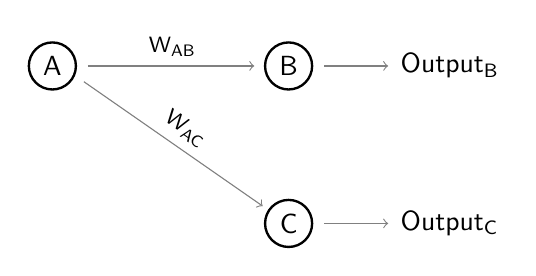
\begin{tikzpicture}[font=\sffamily,shorten >=1pt,->,draw=black!50, node distance=\layersep]
    \tikzstyle{every pin edge}=[<-,shorten <=1pt]
    \tikzstyle{neuron}=[circle,line width=0.3mm,draw=black,minimum size=17pt,inner sep=0pt]
    \tikzstyle{annot} = [text width=4em, text centered]

    \draw[->] (.45,0) -- (2.6,0) node[sloped,midway,above] {\footnotesize W\textsubscript{AB}};
    \draw[->] (.4,-.2) -- (2.7,-1.8) node[sloped,midway,above] {\footnotesize W\textsubscript{AC}};

    \draw[->] (3.45,0) -- (4.3,0) node[right=0cm]{Output\textsubscript{B}};
    \draw[->] (3.45,-2) -- (4.3,-2) node[right=0cm]{Output\textsubscript{C}};
    
    \node[neuron] at (0,0) {A};
    \node[neuron] at (3,0) {B};
    \node[neuron] at (3,-2) {C};
\end{tikzpicture}